% Chapter Template
% !TEX root = ../main.tex
\chapter{SVM - \emph{Support Vector Machine}} % Main chapter title

\label{cap:svm} % Change X to a consecutive number; for referencing this chapter elsewhere, use \ref{ChapterX}

Una SVM (\emph{Support Vector Machine}) è un modello di apprendimento supervisionato associato ad algoritmi largamente utilizzati per l'analisi statistica di dati e il \emph{pattern recognition} (tra cui anche il problema della classificazione).
L'SVM è un modello abbastanza recente; anche se la sua formulazione risale agli anni '60, solo negli ultimi 15/20 anni si è registrato un incremento significativo nell'uso di algoritmi SVM per classificazione \citep{Book_svm}.
La sua fortuna risiede nel fatto che possa essere facilmente applicato a molti campi ed alle sue proprietà ?? in termini di capacità di generalizzazione e robustezza all'aumento del numero di \emph{feature}.%senza stravolgere la semplicità che caratterizza questi classificatori.
\\
Questo capitolo servirà per introdurre la teoria matematica su cui si basa un classificatore SVM e sarà impostato nel seguente modo: si inizierà descrivendo dettagliatamente il modello più semplice di SVM (SVM lineare per classificazione binaria), poi si proseguirà con la descrizione di come è possibile estendere questo modello per una classificazione non-lineare e, infine, verranno introdotte le possibili modifiche che permettono la classificazione multiclasse.
\clearpage

\section{SVM lineare per classificazione binaria}
Dato un \emph{training set} linearmente separabile $(\mathbf{x}_i,y_i)$, $i=1,\ldots,N$, con $\mathbf{x}_i\in\mathbb{R}^d$ e $y_i\in\left\lbrace -1,1\right\rbrace$, l'obiettivo è addestrare un classificatore affinché
\begin{equation}
\label{eq:SVM_lin_bin}
f(\mathbf{x}_i):\twopartdef{>0}{y_i=+1}{< 0}{y_i=-1}
\end{equation}
ovvero $y_if(\mathbf{x}_i)>0$ per una corretta classificazione.
La funzione $f$ è detta \textit{regola di decisione} ed è costruita in modo tale che, preso un qualsiasi \textit{campione incognito} $\mathbf{u}$ da classificare, il valore di $f$ valutato in $\mathbf{u}$ restituisca una stima dell'etichetta $y_u$ da associare. In equazioni:
\begin{equation}
\label{eq:regola_di_decisione}
f\text{ tale che }
\left\{
		\begin{array}{ll}
			\text{Se } f(\mathbf{u})>0 & \mbox{allora } y_u=+1 \\
			\text{Se } f(\mathbf{u})<0 & \mbox{allora } y_u=-1 \\
		\end{array}
	\right.
\end{equation}
\subsection{Hard Margin SVM}
Un insieme di elementi in $\mathbb{R}^d$ è linearmente separabile se esiste almeno un iperpiano (che in generale avrà dimensione $d-1$) in grado di separare, nello spazio vettoriale dei campioni in ingresso, quelli che richiedono un'etichetta positiva da quelli che richiedono un'etichetta negativa. 
\\
Si prenda, per esempio, la situazione proposta in Figura \ref{fig:insieme_lin_separ}: qui si può facilmente evincere che esista almeno un iperpiano (in questo caso una retta) che divida lo spazio in due semispazi, ciascuno dei quali contiene campioni di una sola classe.
\begin{figure}[!ht]
\begin{center}

	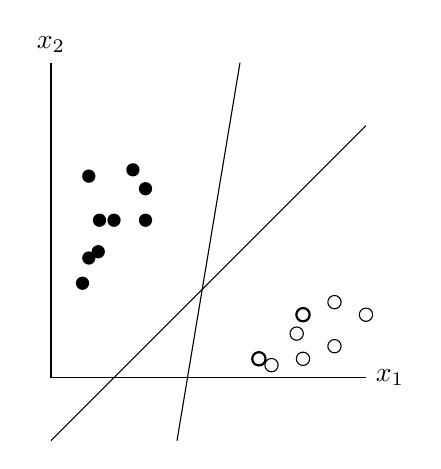
\begin{tikzpicture}[scale=0.8]
	  % Draw axes
	 \draw [] (0,5) node (yaxis) [above] {$x_2$}
	        |- (5,0) node (xaxis) [right] {$x_1$};
	  \draw (0,-1) -- (5,4);
	  \draw (2,-1) -- (3,5);
	  % Draw negative dots
	  	\fill[black] (0.5,1.5) circle (3pt);
	  	\fill[black]   (1.5,2.5)   circle (3pt);
	  	\fill[black] (1,2.5)     circle (3pt);
	  	\fill[black] (0.75,2)    circle (3pt);
	  	\fill[black] (0.6,1.9)   circle (3pt);
	  	\fill[black] (0.77, 2.5) circle (3pt);
	  	\fill[black] (1.5,3)     circle (3pt);
	  	\fill[black] (1.3,3.3)   circle (3pt);
	  	\fill[black] (0.6,3.2)   circle (3pt);
	  % Draw positive dots
  		\draw[black,thick] (4,1)     circle (3pt); 
  		\draw[black,thick] (3.3,.3)  circle (3pt); 
  		\draw[black]     (4.5,1.2) circle (3pt); 
  		\draw[black]     (4.5,.5)  circle (3pt); 
  		\draw[black]     (3.9,.7)  circle (3pt); 
  		\draw[black]     (5,1)     circle (3pt); 
  		\draw[black]     (3.5,.2)  circle (3pt); 
  		\draw[black]     (4,.3)    circle (3pt); 
	\end{tikzpicture}
	
\end{center}
	\caption{\emph{Training set} binario linearmente separabile}
	\label{fig:insieme_lin_separ}
\end{figure}
\\
Il problema nasce dal fatto che possano esistere infiniti iperpiani e la scelta di quale usare per l'addestramento possa avere ripercussioni notevoli sulla fase di classificazione. 
L'SVM risolve questo problema cercando l'iperpiano che massimizza il margine tra i due insiemi di elementi. 
\\
In termini matematici, un iperpiano in $\mathbb{R}^d$ ha forma:
\begin{equation}
\label{eq:iperpiano}
\mathbf{w}\cdot\mathbf{x}+b=0
\end{equation}
dove $\mathbf{w}\in\mathbb{R}^d$ è la normale all'iperpiano e $b/ \vert\vert\mathbf{w}\vert\vert$ è la distanza dell'origine dall'iperpiano.
\\
Alla luce di ciò, si può riscrivere la \textit{regola di decisione} presentata nell'equazione (\ref{eq:regola_di_decisione}) nel seguente modo:
\begin{equation}
\label{eq:regola_di_decisioneSVM}
\left\{
		\begin{array}{ll}
			\text{Se } \mathbf{w}\cdot\mathbf{u}+b>0 & \mbox{allora } y_u=+1 \\
			\text{Se } \mathbf{w}\cdot\mathbf{u}+b<0 & \mbox{allora } y_u=-1 \\
		\end{array}
	\right.
\end{equation}

Dato che $\mathbf{w}\cdot\mathbf{x}+b=0$ e $c\left (\mathbf{w}\cdot\mathbf{x}+b\right )=0$ definiscono la stessa regola di decisione per $c>0$, si ha libertà di scegliere la normalizzazione di $\mathbf{w}$.
In questo caso, si può scegliere il fattore di normalizzazione in modo tale che $\mathbf{w}\cdot\mathbf{x}_i+b\geq 1$ e $\mathbf{w}\cdot\mathbf{x}_i+b\leq-1$, per gli elementi di \emph{training} della prima classe e della seconda rispettivamente.
Per convenienza matematica, dato che $y_i\in\left\lbrace -1,1\right\rbrace$, le due identità precedenti possono essere riscritte nel seguente modo:
\begin{equation}
\label{eq:disq_elementi1}
y_i\left (\mathbf{w}\cdot\mathbf{x}_i+b\right )\geq1,\quad \forall i=1,\ldots,N
\end{equation}
o, analogamente,
\begin{equation}
\label{eq:disq_elementi2}
y_i\left (\mathbf{w}\cdot\mathbf{x}_i+b\right )-1\geq0,\quad \forall i=1,\ldots,N
\end{equation}
con l'uguaglianza valida per gli elementi sul bordo (i punti rossi in Figura \ref{fig:margine}).
\\

\begin{figure}[!ht]
\begin{center}

	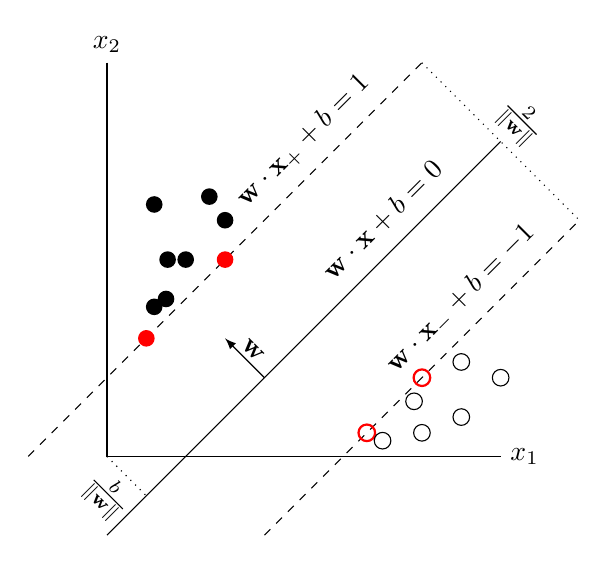
\begin{tikzpicture}
  % Draw axes
 \draw [] (0,5) node (yaxis) [above] {$x_2$}
        |- (5,0) node (xaxis) [right] {$x_1$};
  % Draw line
  \draw (0,-1) -- (5,4); % y=x-1
  \draw[dashed] (-1,0) -- (4,5); % y=x+1
  \draw[dashed] (2,-1) -- (6,3); % y=x-3
%  % Draw labels
  \draw (3.5,3) node[rotate=45] 
        {$\mathbf{w}\cdot \mathbf{x} + b = 0$};
  \draw (2.5,4) node[rotate=45] 
        {$\mathbf{w}\cdot \mathbf{x}_+ + b = 1$};
  \draw (4.5,2) node[rotate=45] 
       {$\mathbf{w}\cdot \mathbf{x}_- + b = -1$};
  % Draw distance
  \draw[dotted] (4,5) -- (6,3);
  \draw (5.25,4.25) node[rotate=-45] {$\frac{2}{\Vert \mathbf{w} \Vert}$};
  \draw[dotted] (0,0) -- (0.5,-0.5);
  \draw (0,-0.5) node[rotate=-45] {$\frac{b}{\Vert \mathbf{w} \Vert}$};
  \draw[-latex] (2,1) -- (1.5,1.5);
  \draw (1.85,1.35) node[rotate=-45] {$\mathbf{w}$};
  % Draw negative dots
  \fill[red] (0.5,1.5) circle (3pt);
  \fill[red]   (1.5,2.5)   circle (3pt);
  \fill[black] (1,2.5)     circle (3pt);
  \fill[black] (0.75,2)    circle (3pt);
  \fill[black] (0.6,1.9)   circle (3pt);
  \fill[black] (0.77, 2.5) circle (3pt);
  \fill[black] (1.5,3)     circle (3pt);
  \fill[black] (1.3,3.3)   circle (3pt);
  \fill[black] (0.6,3.2)   circle (3pt);
  % Draw positive dots
  \draw[red,thick] (4,1)     circle (3pt); 
  \draw[red,thick] (3.3,.3)  circle (3pt); 
  \draw[black]     (4.5,1.2) circle (3pt); 
  \draw[black]     (4.5,.5)  circle (3pt); 
  \draw[black]     (3.9,.7)  circle (3pt); 
  \draw[black]     (5,1)     circle (3pt); 
  \draw[black]     (3.5,.2)  circle (3pt); 
  \draw[black]     (4,.3)    circle (3pt); 
\end{tikzpicture}
	
\end{center}
	\caption{Margine tra i campioni di \emph{training} di due classi linearmente separabili}
	\label{fig:margine}
\end{figure}

Geometricamente, sotto queste ipotesi, si dimostra che il margine risulta essere: 
\begin{equation}
\label{eq:margine}
\dfrac{\mathbf{w}}{\vert\vert\mathbf{w}\vert\vert}\cdot\left (\mathbf{x}_+-\mathbf{x}_-\right )=\dfrac{2}{\vert\vert\mathbf{w}\vert\vert}
\end{equation}
dove $\mathbf{x}_+$ e $\mathbf{x}_-$ sono i campioni delle due classi (rispettivamente) più vicini all'iperpiano separatore (vedi Figura \ref{fig:margine} ed equazione (\ref{eq:disq_elementi2})).
\\
L'obiettivo ora è quindi massimizzare questo valore, che equivale a minimizzare $\vert\vert\mathbf{w}\vert\vert$, il quale, a sua volta, per convenienza matematica, può essere espresso nel seguente termine:
\begin{eqnarray}\nonumber
\label{eq:problema_di_minimizzazione}
&\text{min}\dfrac{1}{2}\vert\vert\mathbf{w}\vert\vert^2\\
&\text{ vincolato a }y_i\left (\mathbf{w}\cdot\mathbf{x}_i+b\right )-1\geq0 \quad \forall i=1,\ldots,N
\end{eqnarray}
%\begin{equation}
%\label{eq:problema_di_minimizzazione}
%\text{min}\dfrac{1}{2}\vert\vert\mathbf{w}\vert\vert^2
%\text{ vincolato a }y_i\left (\mathbf{w}\cdot\mathbf{x}_i+b\right )-1=0
%\end{equation}
\\
%Discorso sul problema della programmazione quadratica.
%(Poiché questi problemi sono già stati ampiamente studiati sia dal punto di vista teorico che da quello applicativo degli algoritmi, possiamo beneficiare immediatamente dei risultati ottenuti nella teoria dell’ottimizzazione. In particolare, questo approccio produce algoritmi computazionalmente efficienti e adattabili a un ampio numero di casi in cui non i dati non sono classificabili senza errore.
%Because it is quadratic, the surface is a paraboloid, with just a single global minimum 
%\\
Essendo questo un problema di calcolo di estremi vincolati si possono usare i \textit{moltiplicatori di Lagrange}, che permettono di lavorare su un problema duale, ovvero l'ottimizzazione (minimizzazione rispetto a $\mathbf{w}$ e a $b$) della seguente funzione:
\begin{equation}
\label{eq:lagrangiana}
\text{min}_{\mathbf{w},b}\text{ }L=\dfrac{1}{2}\vert\vert\mathbf{w}\vert\vert^2-\sum_i\alpha_i\left [y_i\left (\mathbf{w}\cdot\mathbf{x}_i+b\right )-1\right ]
\end{equation}
dove si sottintende, da questo punto in poi, che la sommatoria sia per ogni $i=1,\ldots,N$.
\\
Procedendo con il calcolo del gradiente di $L$ si ottengono i seguenti risultati:
\begin{equation}
\label{eq:deriv_lagrang_rispetto_w}
\dfrac{\partial L}{\partial \mathbf{w}}=\mathbf{w}-\sum_i\alpha_i y_i\mathbf{x}_i=0 \quad\Rightarrow\quad \mathbf{w}=\sum_i\alpha_i y_i\mathbf{x}_i
\end{equation}
\begin{equation}
\label{eq:deriv_lagrang_rispetto_b}
\dfrac{\partial L}{\partial b}=-\sum_i\alpha_iy_i=0 \quad\Rightarrow\quad \sum_i\alpha_iy_i=0
\end{equation}
L'equazione (\ref{eq:deriv_lagrang_rispetto_w}) suggerisce che il vettore $\mathbf{w}$ non sia altro che una combinazione lineare di alcuni vettori di \emph{training} (per alcuni di loro $\alpha_i$ sarà pari a $0$), mentre l'equazione (\ref{eq:deriv_lagrang_rispetto_b}) sarà utile più avanti.

A questo punto si introduce il cosiddetto \textit{problema lagrangiano duale}: invece di \emph{minimizzare} rispetto a $\mathbf{w}$ e $b$, si può \emph{massimizzare} rispetto ad $\alpha$ con vincoli le relazioni ottenute precedentemente per $\mathbf{w}$ e $b$ (equazioni (\ref{eq:deriv_lagrang_rispetto_w}) e (\ref{eq:deriv_lagrang_rispetto_b}))\footnote{Il teorema di Kunh-Tucker assicura che la soluzione di questo problema è la stessa del problema originario; per maggiori informazioni si consulti \citep{Tutorial_burges} e \citep{Libro_SVM2}}.

Dato che l'equazione (\ref{eq:deriv_lagrang_rispetto_w}) restituisce una espressione per $\mathbf{w}$, possiamo sostituire questo risultato nella lagrangiana $L$ (eq.ne (\ref{eq:lagrangiana})), ottenendo:
\begin{eqnarray}\nonumber
\label{eq:lagrangiana_finale1}
&L(\mathbf{w},b)	= \dfrac{1}{2}\left ( \sum_i \alpha_iy_i\mathbf{x}_i \right )\cdot\left (\sum_j\alpha_jy_j\mathbf{x}_j\right )+\\
		&-\sum_i\left [\alpha_iy_i\mathbf{x}_i\cdot\left (\sum_j\alpha_jy_j\mathbf{x}_j\right )\right ]-
		\sum_i\alpha_iy_ib+\sum_i\alpha_i	
\end{eqnarray}
%\begin{equation}
%\label{eq:lagrangiana_finale1}
%L	= \dfrac{1}{2}\left ( \sum_i \alpha_iy_i\mathbf{x}_i \right )\cdot\left (\sum_j\alpha_jy_j\mathbf{x}_j\right )-
%		\sum_i\left [\alpha_iy_i\mathbf{x}_i\cdot\left (\sum_j\alpha_jy_j\mathbf{x}_j\right )\right ]-
%		\sum_i\alpha_iy_ib+\sum_i\alpha_i	
%\end{equation}
A questo punto, cambiando l'ordine delle sommatorie nel secondo membro e notando che il penultimo addendo è sempre nullo (vedi equazione (\ref{eq:deriv_lagrang_rispetto_b})), si ottiene la versione finale della lagrangiana duale: 
\begin{equation}
\label{eq:langrangiana_finale2}
L=\sum_i\alpha_i-\dfrac{1}{2	}\sum_i\sum_j\alpha_i\alpha_jy_iy_j\mathbf{x}_i\cdot\mathbf{x}_j
\end{equation}
L'equazione appena riportata è un problema di programmazione quadratica (\emph{quadratic programmimg}, QP) che assicura l'esistenza e l'unicità di una e una sola soluzione.\\

Per completare il discorso sulla SVM lineare, si consideri nuovamente la \emph{regola di decisione} introdotta nell'equazione (\ref{eq:regola_di_decisioneSVM}). Avendo ora una definizione formale per $\mathbf{w}$, questa può essere riscritta nel seguente modo:
\begin{equation}
\label{eq:regola_di_decisioneSVM_lineare}
\left\{
		\begin{array}{ll}
			\text{Se } \sum_i\alpha_i y_i\mathbf{x}_i\cdot\mathbf{u}+b>0 & \mbox{allora } y_u=+1 \\
			\text{Se } \sum_i\alpha_i y_i\mathbf{x}_i\cdot\mathbf{u}+b<0 & \mbox{allora } y_u=-1 \\
		\end{array}
	\right.
\end{equation}

Il motivo dell'uso di questo espediente matematico risiede nel fatto che adesso sia l'ottimizzazione della lagrangiana (\ref{eq:langrangiana_finale2}) sia la \emph{regola di decisione} (\ref{eq:regola_di_decisioneSVM_lineare}) dipendono esclusivamente da un prodotto scalare tra due vettori, $\mathbf{x}_i\cdot\mathbf{x}_j$ e $\mathbf{x}_i\cdot\mathbf{u}$ rispettivamente, e questo semplificherà notevolmente la trattazione della SVM non lineare. 

\subsection{Soft Margin SVM}
Prima di introdurre l'estensione della SVM che permetta la classificazione non-lineare, è interessante discutere di come sia possibile usare una SVM lineare anche per situazioni in cui il \emph{training set} non sia linearmente separabile.\\
Si prenda, come esempio, la situazione proposta di seguito (Figura \ref{fig:Dataset_nonseparabile}).
 \begin{figure}[!ht]
 \center
\begin{tikzpicture}
%\draw[step=0.5,blue!20,thin] (-1,-1) grid (6,6);
%\draw[step=1,blue!50,thin] (-1,-1) grid (6,6);
  % Draw axes
 \draw [] (0,5) node (yaxis) [above] {$x_2$}
        |- (5,0) node (xaxis) [right] {$x_1$};
  % Draw line
%  \draw (-1,-.25) -- (4,4.75); % y=x-1
%  \draw[dashed] (-1,0) -- (4,5); % y=x+1
%  \draw[dashed] (-1,-0.5) -- (4,4.5); % y=x-3 (x+2)


  % Draw negative dots
  \fill[black] (1.5,1) circle (3pt);
  \fill[black]   (2,1.5)   circle (3pt);%%
  \fill[black] (1,2.5)     circle (3pt);
  \fill[black] (0.75,2)    circle (3pt);
  \fill[black] (0.6,1.9)   circle (3pt);
  \fill[black] (0.77, 2.5) circle (3pt);
  \fill[black] (1.5,3)     circle (3pt);
  \fill[black] (1.3,3.3)   circle (3pt);
  \fill[black] (0.6,3.2)   circle (3pt);
  % Draw positive dots
  \draw[black] (1.5,2)     circle (3pt); 
  \draw[black] (3.3,.3)  circle (3pt); 
  \draw[black]     (4.5,1.2) circle (3pt); 
  \draw[black]     (4.5,.5)  circle (3pt); 
  \draw[black]     (3.9,.7)  circle (3pt); 
  \draw[black]     (5,1)     circle (3pt); 
  \draw[black]     (3.5,.2)  circle (3pt); 
  \draw[black]     (4,.3)    circle (3pt); 
\end{tikzpicture}
    \caption{\emph{Training set} binario non linearmente separabile}
    \label{fig:Dataset_nonseparabile}
  \end{figure}
\\
Si nota chiaramente come, in questo caso, non esista alcun iperpiano separatore. 
Nonostante ciò, modificando leggermente il modello di SVM introdotto fino a questo punto, si può dimostrare che è ancora possibile utilizzare una SVM lineare.\\

La chiave di questo nuovo modello sta nell'introduzione di una \emph{variabile di slack}, in modo tale da rilassare quei vincoli rigidi che non permetterebbero l'uso di una SVM lineare. \\
Precedentemente, i margini erano definiti dai vincoli:
\begin{equation}
\label{eq:vincolo_hard_margin}
y_i\left (\mathbf{x}_i\cdot\mathbf{w}+b \right )\geq1   \quad     y_i\in\left\lbrace-1,1\right \rbrace
\end{equation}
Nella soluzione proposta, invece, sono definiti da:
\begin{equation}
\label{eq:vincolo_soft_margin}
y_i\left (\mathbf{x}_i\cdot\mathbf{w}+b \right )\geq1-\xi_i   \quad    \xi_i\geq0, y_i\in\left\lbrace-1,1\right \rbrace
\end{equation}
La situazione che si è andata a definire, graficamente, appare in Figura \ref{fig:soft_margin}.
 \begin{figure}[!ht]
\center
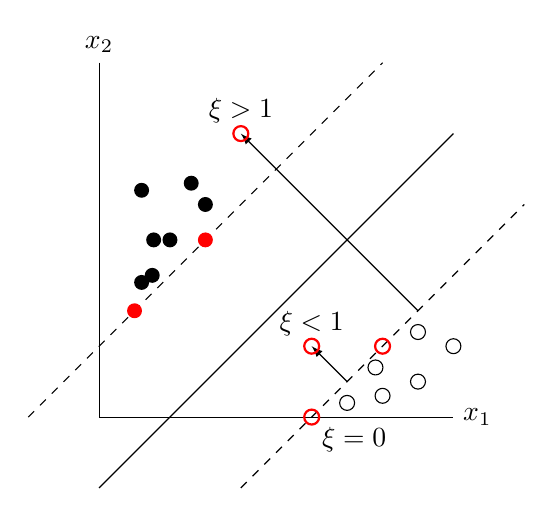
\begin{tikzpicture}[scale=0.9]
%\draw[step=0.5,blue!20,thin] (-1,-1) grid (6,6);
%\draw[step=1,blue!50,thin] (-1,-1) grid (6,6);
  % Draw axes
 \draw [] (0,5) node (yaxis) [above] {$x_2$}
        |- (5,0) node (xaxis) [right] {$x_1$};
  % Draw line
  \draw (0,-1) -- (5,4); % y=x-1
  \draw[dashed] (-1,0) -- (4,5); % y=x+1
  \draw[dashed] (2,-1) -- (6,3); % y=x-3

\draw[-latex](3.5,0.5)--(3,1);  
\draw[-latex](4.5,1.5)--(2,4);  
%  % Draw labels

  % Draw negative dots
  \fill[red] (0.5,1.5) circle (3pt);
  \fill[red]   (1.5,2.5)   circle (3pt);
  \fill[black] (1,2.5)     circle (3pt);
  \fill[black] (0.75,2)    circle (3pt);
  \fill[black] (0.6,1.9)   circle (3pt);
  \fill[black] (0.77, 2.5) circle (3pt);
  \fill[black] (1.5,3)     circle (3pt);
  \fill[black] (1.3,3.3)   circle (3pt);
  \fill[black] (0.6,3.2)   circle (3pt);
  % Draw positive dots
  \draw[red,thick] (4,1)     circle (3pt); 
  \draw[red,thick] (3,0)  circle (3pt)node[below right ,black]{$\xi=0$}; 
  
  \draw[red,thick] (3,1)  circle (3pt)node[above ,black]{$\xi<1$}; 
  \draw[red,thick] (2,4)  circle (3pt)node[above ,black]{$\xi>1$}; 
  \draw[black]     (4.5,1.2) circle (3pt); 
  \draw[black]     (4.5,.5)  circle (3pt); 
  \draw[black]     (3.9,.7)  circle (3pt); 
  \draw[black]     (5,1)     circle (3pt); 
  \draw[black]     (3.5,.2)  circle (3pt); 
  \draw[black]     (4,.3)    circle (3pt); 
\end{tikzpicture}
    \caption{Esempio di soft margin nel caso di un \emph{training set} binario non linearmente separabile}
    \label{fig:soft_margin}
  \end{figure}

Il nuovo vincolo permette al margine funzionale di essere minore di 1. L'errore che si commette è, però, $C\xi_i$, sia per i punti che ricadrebbero nella parte corretta dell'iperpiano separatore ($0<\xi_i\leq1$), sia per quelli che sarebbero nel lato sbagliato ($\xi_i>1$).
Si sono, quindi, "rilassati" i vincoli in modo tale da classificare dati non-separabili, con una penalità linearmente proporzionale all'entità dell'errore commesso sul \emph{training set}.\\

Il nuovo problema di ottimizzazione è il seguente:
\begin{eqnarray}
\label{eq:ottimizzazione_softmargin}
&\text{min }\dfrac{1}{2}\vert\vert\mathbf{w}\vert\vert^2+C\sum_i\xi_i\\
&\text{vincolato a }&y_i\left (\mathbf{x}_i\cdot\mathbf{w}+b \right )\geq1-\xi_i\\
&& \xi_i\geq0, \quad \forall i=1,\ldots,N
\end{eqnarray}
La costante $C$ (con $C\geq0$) gestisce il compromesso fra la minimizzazione dei due contributi alla funzione obiettivo: se $C=0$ gli errori sul \emph{training set} non sono penalizzati; se $C$ è molto grande, il termine legato al margine è minoritario e gli errori sul \emph{training set} sono molto penalizzati.
\\
Allo stesso modo del caso lineare, possono essere usati i moltiplicatori di Lagrange; la funzione da ottimizzare quindi è la seguente:
\begin{equation}
\label{eq:lagrangiana_sofmargin}
L=\dfrac{1}{2}\vert\vert\mathbf{w}\vert\vert^2+C\sum_i\xi_i+\sum_i\alpha_i\left [1-\xi_i-y_i\left (\mathbf{x}_i\cdot\mathbf{w}+b \right )\right ]-\sum_i\beta_i\xi_i
\end{equation}
dove $\beta_i$ sono i moltiplicatori di Lagrange necessari per vincolare la positività della \emph{variabile slack}.	
\\

\'E interessante notare come l'applicazione di una soft-margin SVM possa avere prestazioni migliori della hard-margin SVM anche per dataset linearmente separabili. Per chiarificarne il motivo, un esempio è riportato nella figura successiva: il \emph{training set} permetterebbe l'uso di una hard-margin SVM, ma il risultato  avrebbe un margine piuttosto limitato, confrontato con quello che si otterrebbe in caso di soft-margin SVM. \\
 \begin{figure}[!ht]
 \centering
 \subfigure[Hard Margin SVM]
   {
		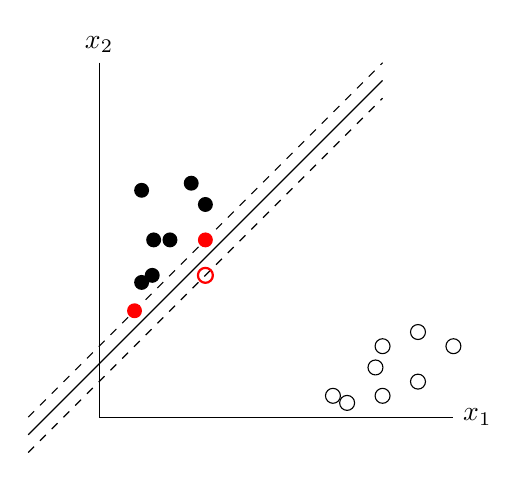
\begin{tikzpicture}[scale=.9]
  % Draw axes
 \draw [] (0,5) node (yaxis) [above] {$x_2$}
        |- (5,0) node (xaxis) [right] {$x_1$};
  % Draw line
  \draw (-1,-.25) -- (4,4.75); % y=x-1
  \draw[dashed] (-1,0) -- (4,5); % y=x+1
  \draw[dashed] (-1,-0.5) -- (4,4.5); % y=x-3 (x+2)

  \fill[red] (0.5,1.5) circle (3pt);
  \fill[red]   (1.5,2.5)   circle (3pt);
  \fill[black] (1,2.5)     circle (3pt);
  \fill[black] (0.75,2)    circle (3pt);
  \fill[black] (0.6,1.9)   circle (3pt);
  \fill[black] (0.77, 2.5) circle (3pt);
  \fill[black] (1.5,3)     circle (3pt);
  \fill[black] (1.3,3.3)   circle (3pt);
  \fill[black] (0.6,3.2)   circle (3pt);
  % Draw positive dots
  \draw[red,thick] (1.5,2)     circle (3pt); 
   \draw[black] (4,1)     circle (3pt);
  \draw[black] (3.3,.3)  circle (3pt); 
  \draw[black]     (4.5,1.2) circle (3pt); 
  \draw[black]     (4.5,.5)  circle (3pt); 
  \draw[black]     (3.9,.7)  circle (3pt); 
  \draw[black]     (5,1)     circle (3pt); 
  \draw[black]     (3.5,.2)  circle (3pt); 
  \draw[black]     (4,.3)    circle (3pt); 
\end{tikzpicture}   
   }
 \hspace{4mm}
 \subfigure[Soft Margin SVM]
   {
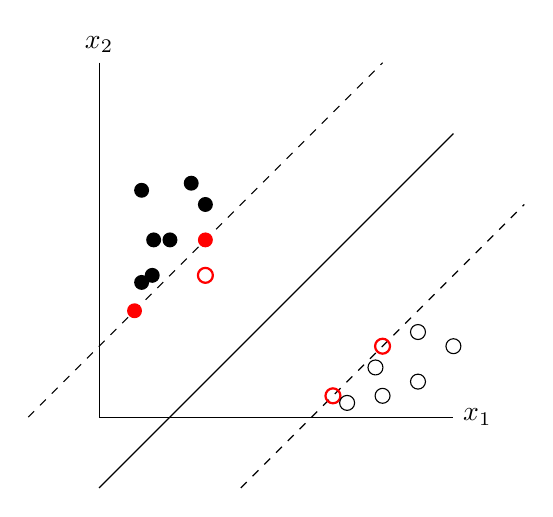
\begin{tikzpicture}[scale=.9]
  % Draw axes
 \draw [] (0,5) node (yaxis) [above] {$x_2$}
        |- (5,0) node (xaxis) [right] {$x_1$};
  % Draw line
  \draw (0,-1) -- (5,4); % y=x-1
  \draw[dashed] (-1,0) -- (4,5); % y=x+1
  \draw[dashed] (2,-1) -- (6,3); % y=x-3

  \fill[red] (0.5,1.5) circle (3pt);
  \fill[red]   (1.5,2.5)   circle (3pt);
  \fill[black] (1,2.5)     circle (3pt);
  \fill[black] (0.75,2)    circle (3pt);
  \fill[black] (0.6,1.9)   circle (3pt);
  \fill[black] (0.77, 2.5) circle (3pt);
  \fill[black] (1.5,3)     circle (3pt);
  \fill[black] (1.3,3.3)   circle (3pt);
  \fill[black] (0.6,3.2)   circle (3pt);
  % Draw positive dots
    \draw[red,thick] (4,1)     circle (3pt); %da aggiungere
  \draw[red,thick] (3.3,.3)  circle (3pt); 
  \draw[red,thick] (1.5,2)     circle (3pt); 
 
  \draw[black]     (4.5,1.2) circle (3pt); 
  \draw[black]     (4.5,.5)  circle (3pt); 
  \draw[black]     (3.9,.7)  circle (3pt); 
  \draw[black]     (5,1)     circle (3pt); 
  \draw[black]     (3.5,.2)  circle (3pt); 
  \draw[black]     (4,.3)    circle (3pt); 
\end{tikzpicture}   
   }
 \caption{Confronto tra Hard Margin SVM e Soft Margin SVM nel caso di un training set binario linearmente separabile}
 \end{figure}
 
\section{SVM non lineare per classificazione binaria}
Nonostante l'introduzione della variante Soft-Margin della SVM possa rimuovere l'ipotesi restrittiva di separabilità lineare del \emph{training set}, può capitare che anche questa strategia sia difficilmente applicabile o produca risultati non soddisfacenti (si rimanda al Capitolo \ref{cap:prestazioni} dove si discuterà come avere una stima delle prestazioni di un classificatore).
\\

L'intento della classificazione SVM non-lineare è quello di trasformare lo spazio dei vettori di \emph{training} non linearmente separabili $\mathbb{R}^d$ in uno spazio $\mathcal{H}$ (la cui dimensionalità sarà maggiore di $d$ o anche, potenzialmente, infinita) in cui i campioni siano disposti in modo tale da permettere l'utilizzo di una SVM lineare. Questo passo si giustifica tramite il \emph{Teorema di Cover sulla separabilità}, il quale afferma che un problema di classificazione complesso, formulato attraverso una trasformazione non-lineare dei dati in uno spazio ad alta dimensionalità, ha maggiore probabilità di essere linearmente separabile che in uno spazio a bassa dimensionalità.
\\
Si ricerca quindi una funzione di trasformazione:
\begin{equation}
\label{eq:funzione_di_trasformazione}
\Phi:\mathbb{R}^d\rightarrow\mathcal{H}
\end{equation}
Graficamente, in Figura \ref{fig:funzione_di_trasformazione} è riportato un esempio della situazione in esame.
 \begin{figure}[!ht]
\begin{tikzpicture}[x=1cm,y=1cm]
%\draw[color=gray!20] (0,0) grid (6,6);
%\draw[color=gray!20] (7,0) grid (13,6);
 
\draw[] (0,0) -- (5.5,0) node[right]{$x_1$};
\draw[] (0,0) -- (0,5) node[above]{$x_2$}; 
 
\fill[] (0,0) circle (3pt);
\fill[] (3,3)   circle (3pt); 
 
\draw[] (0,3) circle (3pt);
\draw[] (3,0)   circle (3pt); 
 
\draw[] (7,0) -- (5.5+7,0) node[right]{$x_1$};
\draw[] (0+7,0) -- (0+7,5) node[above]{$x_2$}; 
 \draw[](7,0)--(4+7,4)node[above]{$x_3$};
 

 \draw[-latex] 
 (4,4.5) .. controls (6,4.5) and (8,3.5) ..
 (8,3.5)node [above,pos=.4] {$\phi$};
 
 \fill[] (7,0) circle (3pt);
\fill[] (12,2)   circle (3pt); 
 
\draw[] (10,2) circle (3pt);
\draw[] (9,4)   circle (3pt); 

\draw[dashed] (10,2) --+(0,-2);
\draw[dashed] (9,4)  --+(0,-2);
  \end{tikzpicture}
    \caption{Trasformazione dello spazio delle \emph{feature} in uno spazio munito di prodotto scalare ed avente dimensione maggiore. Cerchi pieni e vuoti indicano campioni di training di due classi}
    \label{fig:funzione_di_trasformazione}
  \end{figure}
\\
Alla luce di ciò, la lagrangiana (\ref{eq:langrangiana_finale2}), per la fase di addestramento, e la \emph{regola di decisione} (\ref{eq:regola_di_decisioneSVM_lineare}), per la fase di classificazione, possono essere riscritte come segue:
\begin{equation}
\label{eq:lagrangiana_con_funzione_di_trasformazione}
L=\sum_i\alpha_i-\dfrac{1}{2}\sum_i\sum_j\alpha_i\alpha_jy_iy_j\Phi(\mathbf{x}_i)\cdot\Phi(\mathbf{x}_j)
\end{equation}
\begin{equation}
\label{eq:regola_di_decisione_con_funzione_di_trasformazione}
f(\mathbf{u})=\sum_i\alpha_iy_i\Phi(\mathbf{x}_i)\cdot\Phi(\mathbf{u})+b
\end{equation}
Come già accennato in precedenza, operativamente, entrambe le due fasi sono caratterizzate solo dal prodotto scalare dei vettori trasformati; questo suggerisce che non sia necessaria la conoscenza di $\Phi$, in quanto è sufficiente definire un \emph{kernel}:
\begin{equation}
\label{eq:kernel_trick}
K:\mathbb{R}^d\times\mathbb{R}^d\rightarrow\mathbb{R}\quad\text{tale che}\quad K(\mathbf{x},\mathbf{y})=\Phi(\mathbf{x})\cdot\Phi(\mathbf{y})
\end{equation}
Esistono condizioni necessari e sufficienti affinché una data funzione $K$ sia un \emph{kernel}, ovvero affinchè esistano uno spazio $\mathcal{H}$ e una funzione di trasformazione $\Phi$, tali che valga l'equazione (\ref{eq:kernel_trick}) per $\mathbf{x},\mathbf{y}\in\mathbb{R}^d$. \\
La condizioni di Mercer sono condizioni necessarie e sufficienti per definire per quali famiglie di \emph{kernel} $K$ esiste la coppia $\left\lbrace\mathcal{H},\Phi\right\rbrace$ con le proprietà presentate precedentemente.\\
\begin{teorema}
Sia $K(\mathbf{x},\mathbf{y})$ una funzione continua che può essere espansa nella serie
\begin{equation}
\label{eq:condizioni_di_Mercer1}
K(\mathbf{x},\mathbf{y})=\sum_{i=1}^\infty\Phi(\mathbf{x})_i\cdot\Phi(\mathbf{y})_i
\end{equation}
Affinché tale espansione sia valida e per la sua convergenza assoluta, è necessario e sufficiente che la condizione
\begin{equation}
\label{eq:condizioni_di_Mercer2}
\int\int K(\mathbf{x},\mathbf{y})g(\mathbf{x})g(\mathbf{y})d\mathbf{x}d\mathbf{y}\geq0
\end{equation}
sia vera per ogni $g(\cdot)$ che soddisfano
\begin{equation}
\label{eq:}
\int g^2(\mathbf{x})d\mathbf{x}<\infty
\end{equation}
\end{teorema}

Questo espediente matematico è detto \textbf{\emph{kernel trick}} in quanto, dato un \emph{kernel} che soddisfi tali condizioni, un classificatore SVM risulta identificato dal \emph{kernel} stesso, senza alcuna necessità di definire esplicitamente né $\Phi$ né $\mathcal{H}$.
\\
Per completezza, vengono riportati ora i problemi di ottimizzazione della lagrangiana e la \emph{regola di decisione} usando il \emph{kernel trick}:
\begin{equation}
\label{eq:lagrangiana_con_kernel}
L=\sum_i\alpha_i-\dfrac{1}{2}\sum_i\sum_j\alpha_i\alpha_jy_iy_jK(\mathbf{x}_i,\mathbf{x}_j)
\end{equation}
\begin{equation}
\label{eq:regola_di_decisione_con_kernel}
f\mathbf{u})=\sum_i\alpha_iy_iK(\mathbf{x}_i,\mathbf{u})+b
\end{equation}
Alcuni dei \emph{kernel} più famosi e usati sono i seguenti:
\begin{itemize}
\item \textbf{Polinomiale}: $K(\mathbf{x},\mathbf{y})=\left (1+\mathbf{x}\cdot\mathbf{y}\right )^d$ con $d>0$
\item \textbf{Radiale Gaussiano} (RBF):  $K(\mathbf{x},\mathbf{y})=\exp\left (-\dfrac{\vert\vert\mathbf{x}-\mathbf{y}\vert\vert^2}{2\sigma^2}\right )$ il quale introduce una dimensione dello spazio delle \emph{feature} trasformate infinita.
\end{itemize}
\section{Estensioni multiclasse}
Un problema con più classi si affronta mediante SVM esprimendolo come combinazione di problemi binari. Assumendo di operare con $C$ classi, tale operazione si effettua tipicamente in due modi possibili:
\begin{itemize}
\item l'approccio \emph{one-against-one} (OAO) calcola mediante SVM binaria una \emph{regola di decisione} $f_{ij}$ per ogni coppia di classi, per un totale di $C(C-1)/2$ funzioni discriminanti, e classifica un campione incognito $\mathbf{u}\in\mathbb{R}^d$ mediante "votazione" (se $f_{ij}(\mathbf{u})>0$ si dà un voto alla classe $i$-esima, altrimenti alla $j$-esima; si assegna infine $\mathbf{u}$ alla classe che ha ricevuto più voti);
\item l'approccio \emph{one-against-all} (OAA) calcola mediante SVM binaria una \emph{regola di decisione} $f_{i}$ per ogni decisione del tipo "classe $i$ contro classe non-$i$", per un totale di $C$ funzioni discriminanti e assegna $\mathbf{u}\in\mathbb{R}^d$ alla classe $i$-esima se $f_i(\mathbf{u})\geq f_j(\mathbf{u})$ per ogni $j=1,\ldots,C$ con $i\neq j$.
\end{itemize}


%
%\chapter{Risultati sperimentali} % Main chapter title
%
%\label{chapter_Risultati_sperimentali} % Change X to a consecutive number; for referencing this chapter elsewhere, use \ref{ChapterX}
%
%\lhead{Capitolo \ref{chapter_Risultati_sperimentali}. \emph{Risultati sperimentali}} % Change X to a consecutive number; this is for the header on each page - perhaps a shortened title
%
%
%In questo capitolo verranno presentati tre casi di studio e verrà fatta un analisi delle variazioni di prestazioni al variare dei parametri dell’algoritmo  HOG, evidenziando i valori ottimali. 
%Successivamente verranno presentati i risultati ottenuti valutando anche i punti in cui questo algoritmo non ha dato risultati soddisfacenti, cercando di esporre le cause che hanno generato questi errori.
%
%\clearpage
%
%\section{Descrizione dei dataset}
%In questa tesi sono stati analizzati tre casi rilevanti, tutti relativi alla classificazione dell'area urbana di Amiens (Francia).  Si tratta di un problema di classificazione interessante in quanto le regioni coinvolte sono caratterizzate da aree omogenee (come corsi d'acqua), strutture geometriche ben definite (come edifici e strade) e zone di suolo con pattern regolari (come campi coltivabili e non).\\
%Il \emph{dataset} per ogni esperimento è costituito dall'immagine telerilevata, dalla mappa di \emph{training} e dalla mappa di \emph{testing}.
%Le immagini telerilevate sono state acquisite dal sensore passivo \textsc{SPOT5 HRG} con risoluzione spettrale a tre canali, corrispondenti alle lunghezze d'onda del verde (G, $495–570\text{ } nm$), del rosso (R, $620–750\text{ } nm$) e dell'infrarosso (NIR, \emph{Near InfraRed} $0.75–1.4\text{ } \mu m$).
% 
%
%\subsection{Amiens 2006 - 5 \textit{m}}
%L'immagine \emph{Amiens6--5m} è stata acquisita nel 2006 e ha risoluzione di $5\text{ }m/\text{pixel}$ coprendo approssimativamente un'area di $10\text{ }km\times11\text{ }km$ ($2000\times2200$ pixel).\\
%L'insieme delle classi $\Omega=\left\lbrace\omega_1,\omega_2,\ldots,\omega_{10}\right\rbrace$ che costituisce questo primo esperimento è il seguente:
%\begin{enumerate}
%\item Area urbana ad altra densità
%\item Area urbana ad bassa densità
%\item Strade
%\item Area verde urbana 
%\item Suolo nudo
%\item Terreno coltivabile
%\item Terreno non coltivabile 
%\item Alberi
%\item Corsi d'acqua
%\item Specchi d'acqua
%\end{enumerate}
%Nella Figura \ref{fig: Amiens65m} vengono presentate le immagini caratterizzanti il primo \emph{dataset}; si osservi con attenzione la composizione dell'immagine di training: INSERIRE DISCORSO SU NUMERO DI PIXEL DI TRAINING PER CLASSI
%
%\clearpage
%\begin{figure}[!ht]
%   \center
%   \subfigure[Immagine telerilevata]{
%      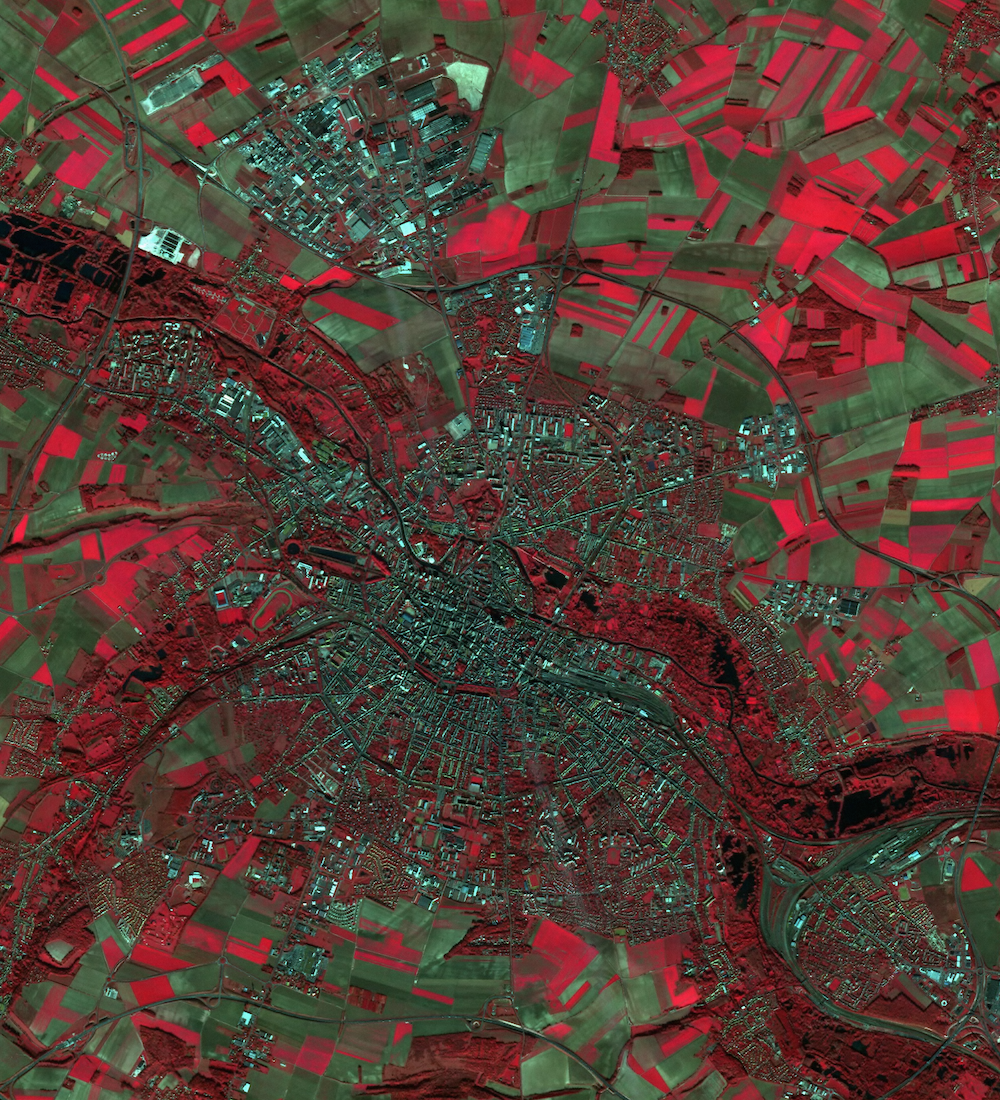
\includegraphics[scale=0.172]{Amiens_2006_SPOT_5m}}\\%pdf0.45
%         \subfigure[Mappa di \emph{training}]{
%      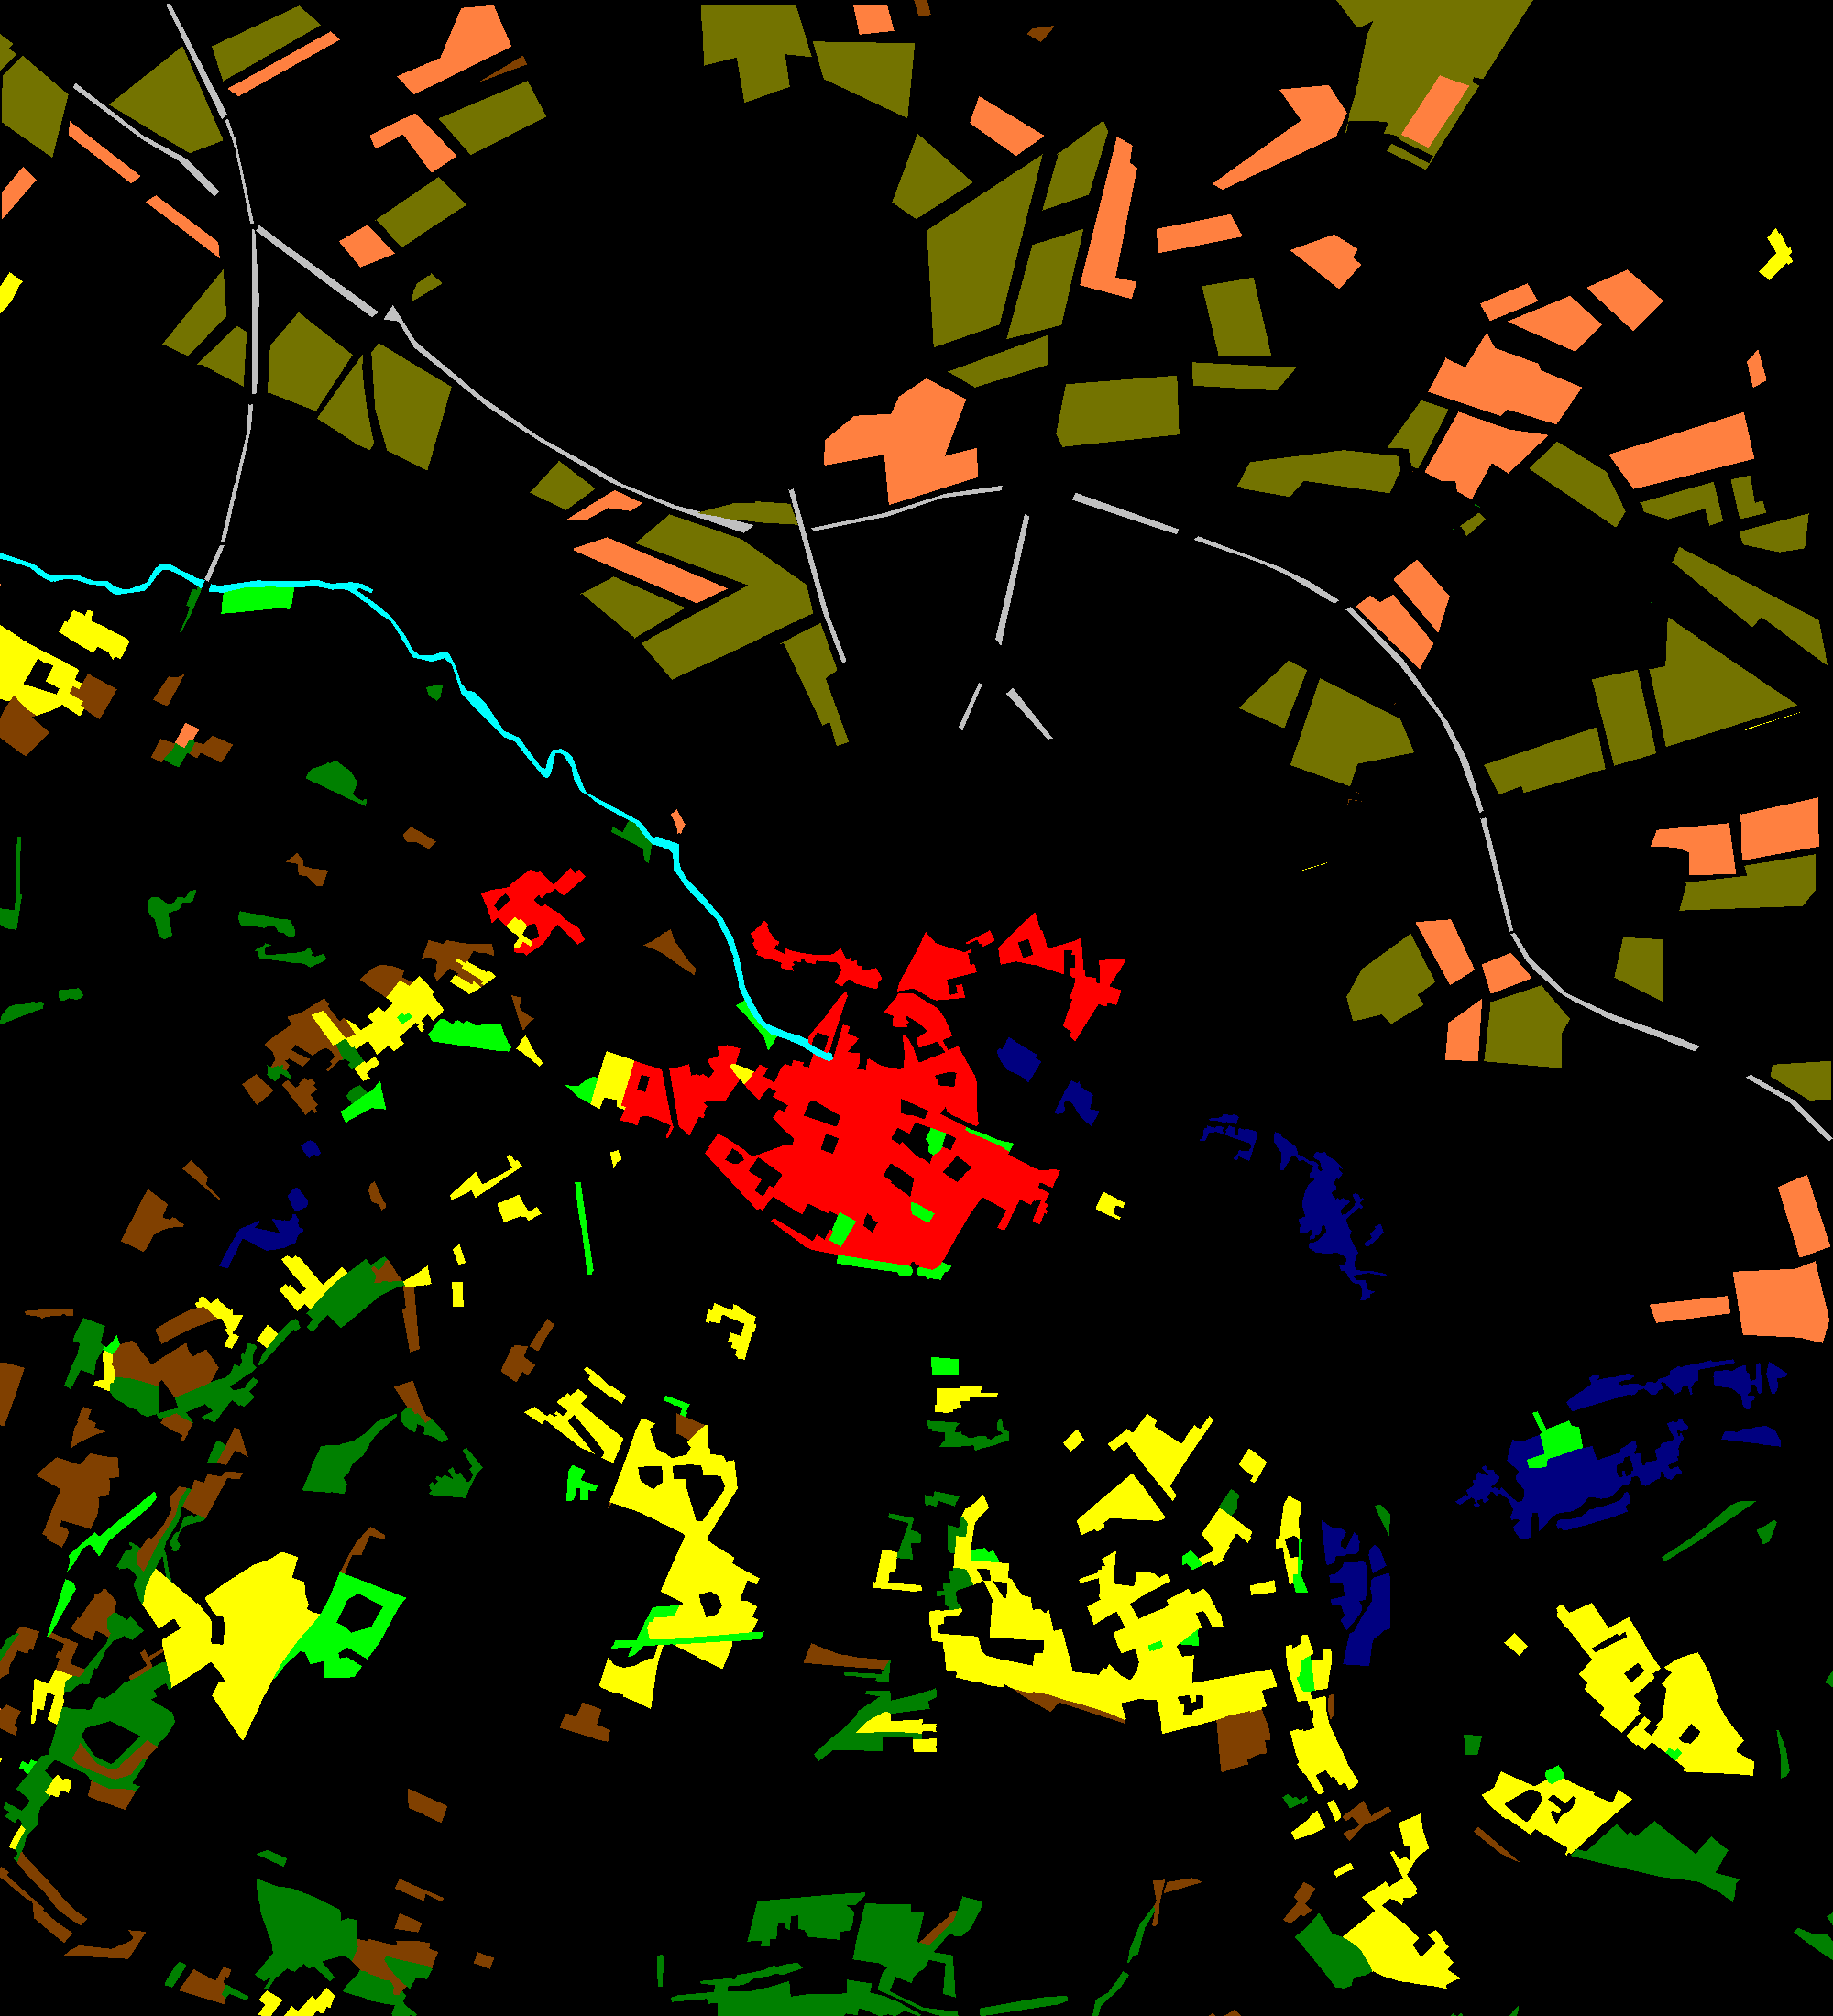
\includegraphics[scale=0.086]{GT_Amiens2006_5m_10classes_TR}}
%     \hspace{4mm}
%    \subfigure[Leggenda classi della mappa di \emph{training}]{
%      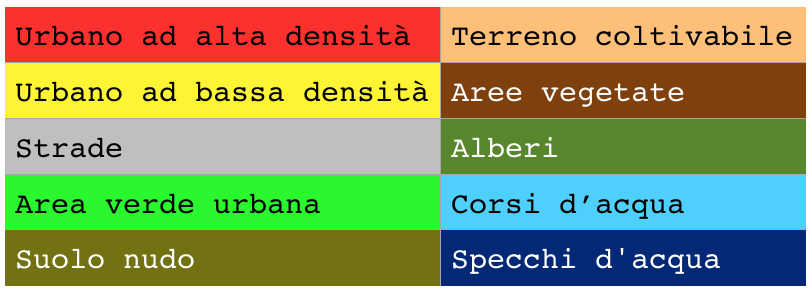
\includegraphics[scale=0.5]{Leggenda_2006_10classi}}
%    \caption{Dataset con immagine RBG in falso colore ($2000\times2200$ pixel) acquisita su Amiens (Francia) dal sensore \textsc{SPOT5 HRG}}
%    \label{fig: Amiens65m}
%  \end{figure}
%
%
%\clearpage
%\subsection{Amiens 2006 - 2.5 \textit{m}}
%L'immagine \emph{Amiens6--2.5m} è stata acquisita nel 2006 e ha risoluzione di $2.5\text{ }m/\text{pixel}$ coprendo sempre approssimativamente un'area di $10\text{ }km\times11\text{ }km$ ($4001\times4400$ pixel).\\
%L'insieme delle classi $\Omega=\left\lbrace\omega_1,\omega_2,\ldots,\omega_{7}\right\rbrace$ che costituisce il secondo \emph{dataset} è il seguente:
%\begin{enumerate}
%\item Edifici
%\item Strade e marciapiedi
%\item Aree vegetate
%\item Suolo nudo
%\item Terreno coltivabile
%\item Alberi
%\item Acqua
%\end{enumerate}
%Nella Figura \ref{fig: Amiens65m} vengono presentate le immagini caratterizzanti il primo \emph{dataset}; si osservi con attenzione la composizione dell'immagine di training: INSERIRE DISCORSO SU NUMERO DI PIXEL DI TRAINING PER CLASSI
%\clearpage
%\begin{figure}[!ht]
%   \center
%   \subfigure[Immagine telerilevata]{
%      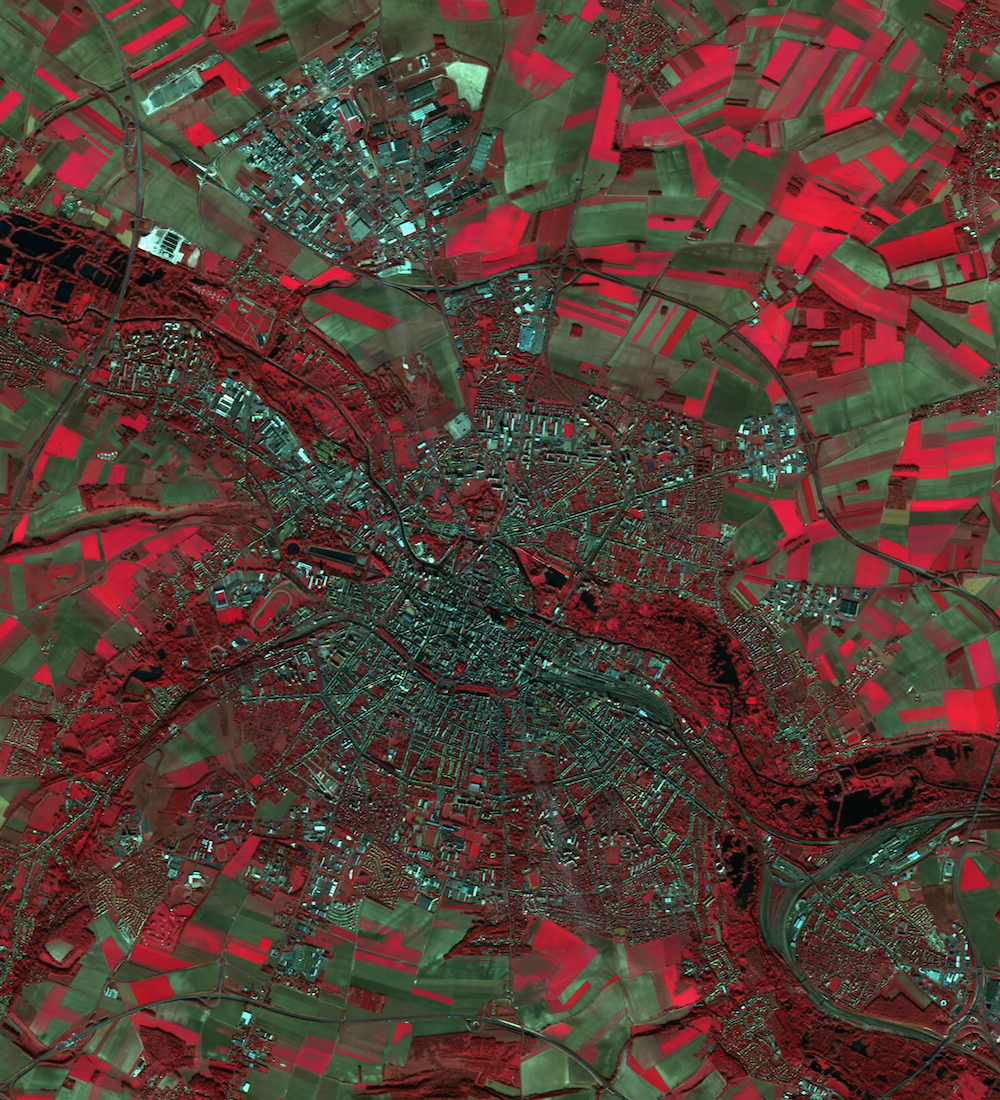
\includegraphics[scale=0.086]{Amiens_2006_SPOT_2_5m}}\\%pdf0.45
%         \subfigure[Mappa di \emph{training}]{
%      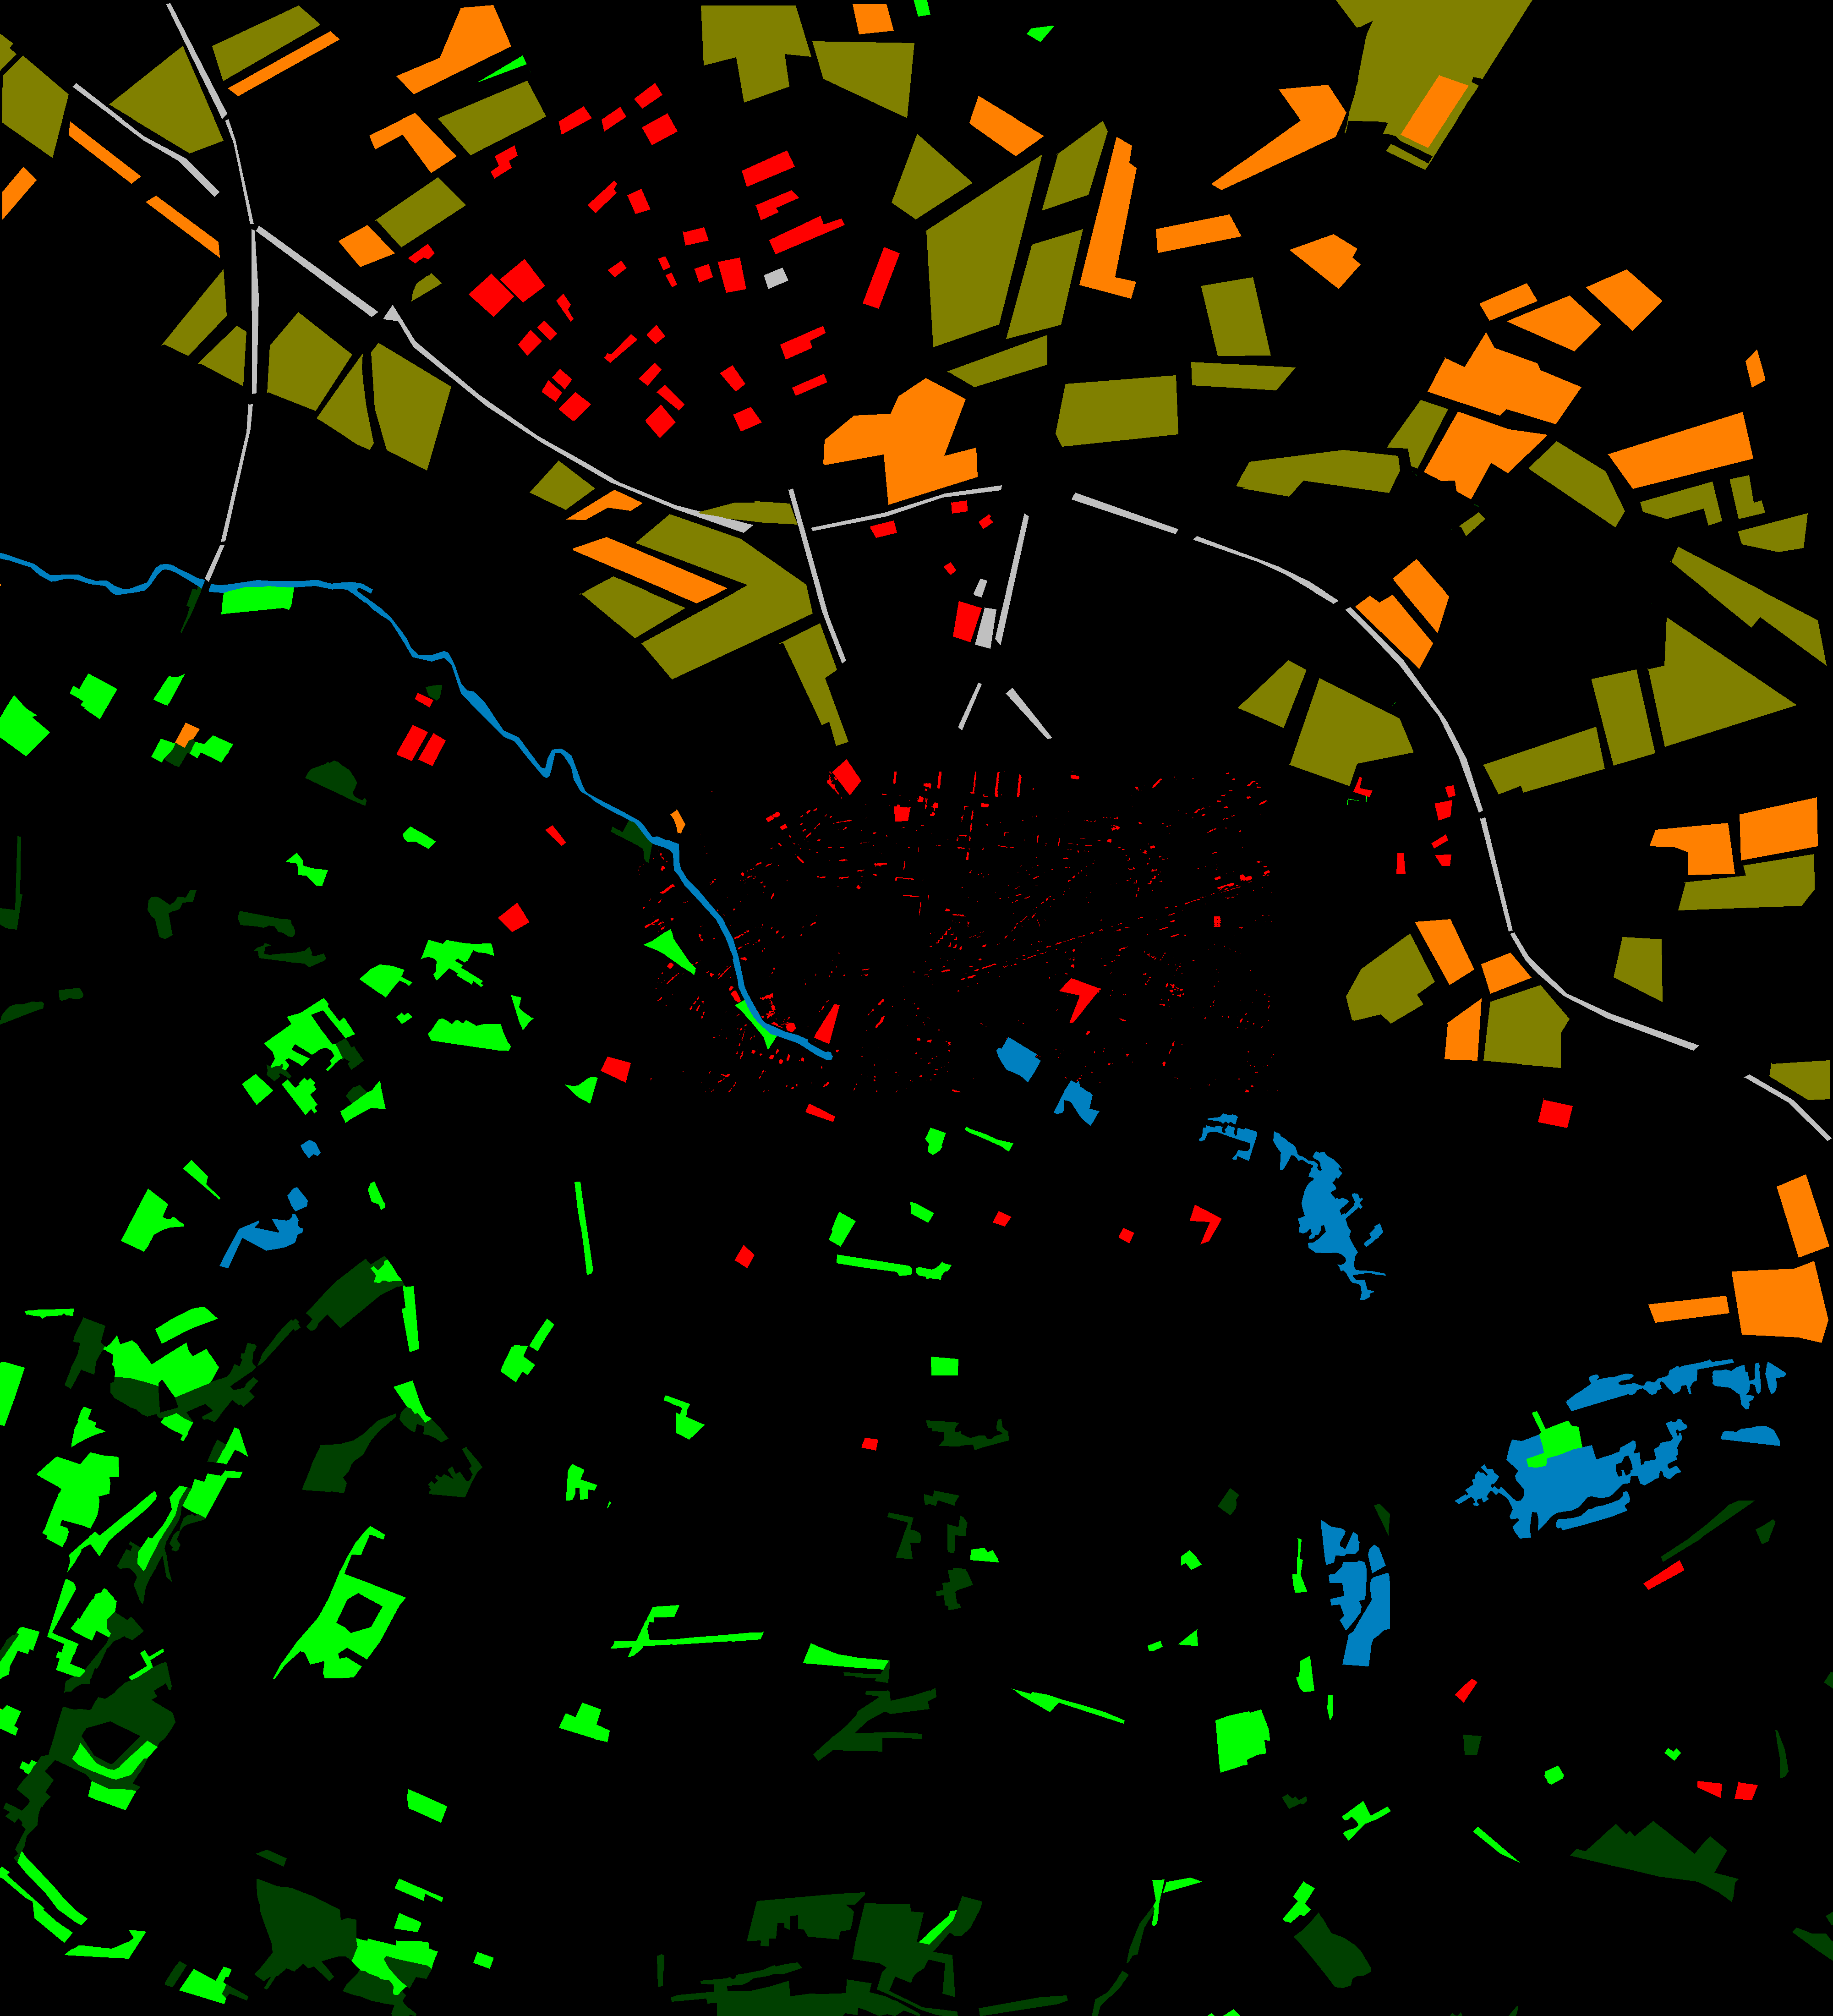
\includegraphics[scale=0.043]{GT_Amiens2006_2_5m_7classes_TR}}
%     \hspace{4mm}
%    \subfigure[Leggenda classi della mappa di \emph{training}]{
%      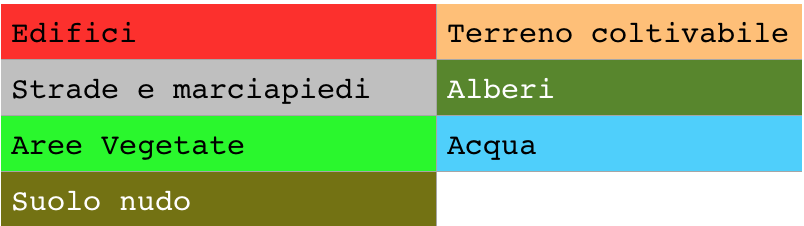
\includegraphics[scale=0.5]{Leggenda_7classi}}
%    \caption{Dataset con immagine RBG in falso colore ($2000\times2200$ pixel) acquisita su Amiens (Francia) dal sensore \textsc{SPOT5 HRG}}
%    \label{fig: Amiens65m}
%  \end{figure}
%
%
%\clearpage
